% Provenance (never printed): cycle 4 SVT/physique, "La planete Terre,
% l'environnement": uneven heating of the Earth, movements of the
% atmosphere, the global circulation and the climate zones; see
% sources/book1/PROVENANCE.md. Book 1, grade 8, chapter 2.
% Vocabulary guard: owns convection cell (atmospheric, descriptive), sea
% breeze and land breeze, the global winds, the global circulation. The
% Coriolis effect is told as "the Earth's rotation deflects"; Hadley and
% Ferrel cells and the intertropical convergence zone are named in prose
% only (Book 3 owns them); mantle convection is Book 2's.
\chapter{Wind en de algemene circulatie}\label{ch:g8:winds-global-circulation}

Eeuwenlang vertrouwden zeilschepen die uit de havens van Europa en Afrika
naar Amerika vertrokken op een gestage wind uit het oosten, die aan
weerszijden van de \omterm{def:g3:continents-and-oceans:equator}{evenaar} waait en hen over de Atlantische \omterm{def:g2:water-on-earth:ocean}{Oceaan}
voerde. Zeelieden over de hele wereld kenden hem, en de vroege handel met
Amerika hing ervan af: het is de \emph{passaatwind}. Ook nu nog gebruiken
vrachtschepen de \omterm{def:g8:winds-global-circulation:global-winds}{passaatwinden}, en de zeestromingen die ze aandrijven, om
hun reizen te bekorten.
% ledger: nos:trade-winds

\begin{omfigure}
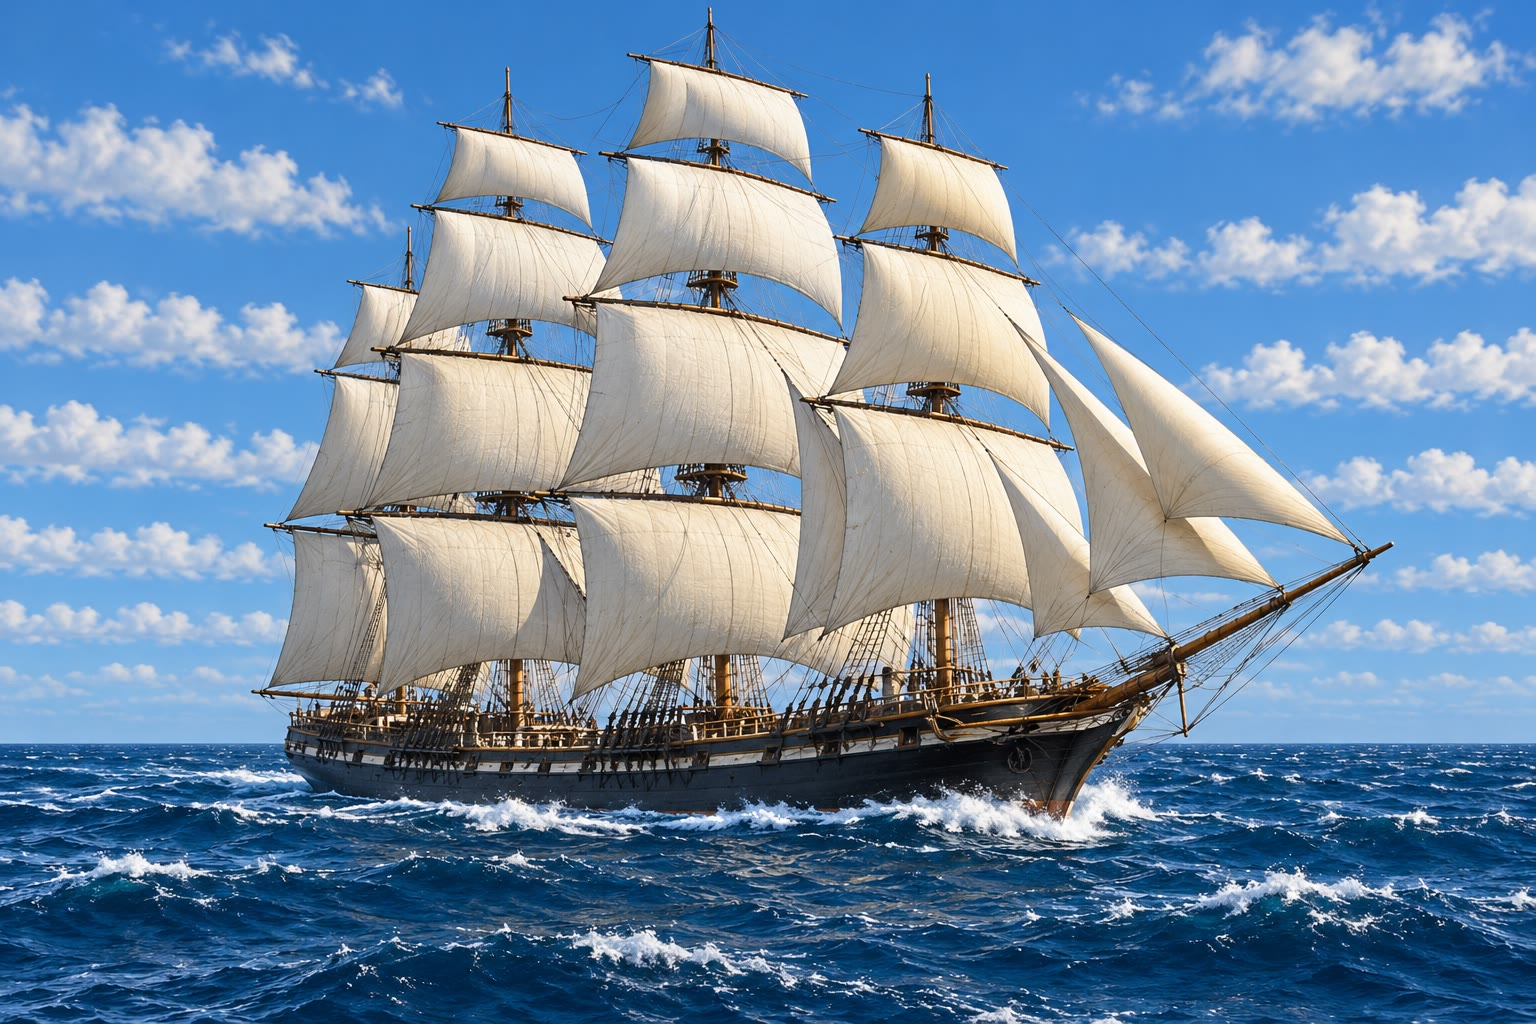
\includegraphics[width=0.62\linewidth]{images/book1/ai/g8-sailing-ship.jpg}

{\small Een zeilschip dat op open \omterm{def:g2:water-on-earth:ocean}{zee} voor een gestage wind uit vaart
(door AI gegenereerde illustratie van een algemene scène).}
\label{fig:g8:winds-global-circulation:ship}
\end{omfigure}

Waarom waait de passaatwind uit het oosten, en altijd op dezelfde plaatsen?
Waarom liggen er \omterm{def:g5:weather-and-climate:desert}{woestijnen} bij de \omterm{def:g5:weather-and-climate:tropics}{keerkringen} en \omterm{def:g5:weather-and-climate:rainforest}{regenwouden} bij de
\omterm{def:g3:continents-and-oceans:equator}{evenaar}? Het antwoord begint bij de Zon.

\begin{recall}
Wind is bewegende lucht (de natuurkundeboeken). Lucht drukt op alles wat
ze raakt, en de druk neemt af met de hoogte (\cref{ch:g8:the-atmosphere}).
Het \omterm{def:g1:watching-the-weather:weather}{weer} speelt zich af in de \omterm{def:g8:the-atmosphere:layers}{troposfeer}, de onderste laag van de
atmosfeer. De Aarde heeft \omterm{def:g5:weather-and-climate:climate-zone}{klimaatzones}: warm en nat bij de \omterm{def:g3:continents-and-oceans:equator}{evenaar}, met
\omterm{def:g5:weather-and-climate:rainforest}{regenwouden}; hete en droge \omterm{def:g5:weather-and-climate:desert}{woestijnen} bij de \omterm{def:g5:weather-and-climate:tropics}{keerkringen}; gematigde en dan
koude zones naar de \omterm{def:g3:continents-and-oceans:poles}{polen} toe (\cref{ch:g5:weather-and-climate}).
\end{recall}

\section{De Zon verwarmt de Aarde ongelijk}

Om 12 uur 's middags op de dag van een equinox staat de Zon recht boven de
\omterm{def:g3:continents-and-oceans:equator}{evenaar}. Haar stralen komen daar steil aan en vallen op een klein stuk
grond. Verder naar het noorden of het zuiden komen dezelfde stralen schuin
aan en worden ze over een groter stuk verspreid: elke vierkante meter
krijgt minder van hun energie. Op een breedte van \ang{60} bedekt dezelfde
bundel twee keer zoveel grond als bij de \omterm{def:g3:continents-and-oceans:equator}{evenaar}, dus krijgt elke
vierkante meter maar de helft.
% ledger: (geometry: figdata/grade-8/sunlight_spread.py, spread = 1/cos(latitude))

\begin{omfigure}
\begin{tikzpicture}[font=\footnotesize]
  \def\R{2.6}\def\w{0.2}
  \fill[blue!10] (0,0) circle (\R);
  \draw (0,0) circle (\R);
  \draw[black!50] (-\R,0) -- (\R,0);
  \draw[black!40, dashed] (0,0) -- (60:\R);
  \draw[black!40] (0,0) ++(0:0.7) arc (0:60:0.7);
  \node at (25:0.95) {\ang{60}};
  \node[anchor=east, black!60] at (-\R-0.05,0) {evenaar};
  % beam at the equator: rays between y = -w and y = w
  \foreach \y in {-0.2,-0.1,0,0.1,0.2} {
    \pgfmathsetmacro{\x}{sqrt(\R*\R-\y*\y)}
    \draw[orange!80!black, -{Stealth[length=1.6mm]}] (6.2,\y) -- (\x+0.03,\y);}
  \draw[omThm, line width=2.2pt] ({sqrt(\R*\R-0.35*0.35)},-0.35) arc ({asin(-\w/\R)}:{asin(\w/\R)}:\R);
  % beam near 60 degrees: rays between y = R sin 60 - w and + w
  \pgfmathsetmacro{\yc}{\R*sin(60)}
  \foreach \d in {-0.2,-0.1,0,0.1,0.2} {
    \pgfmathsetmacro{\y}{\yc+\d}
    \pgfmathsetmacro{\x}{sqrt(\R*\R-\y*\y)}
    \draw[orange!80!black, -{Stealth[length=1.6mm]}] (6.2,\y) -- (\x+0.03,\y);}
  \draw[omThm, line width=2.2pt] ({sqrt(\R*\R-(\yc-\w)^2)},\yc-\w) arc ({asin((\yc-\w)/\R)}:{asin((\yc+\w)/\R)}:\R);
  \node[anchor=west, align=left] at (6.3,0) {dezelfde bundel\\op een klein stuk};
  \node[anchor=west, align=left] at (6.3,\yc) {dezelfde bundel verspreid\\over twee keer zoveel grond};
\end{tikzpicture}

{\small Twee identieke bundels zonlicht om 12 uur 's middags op een
equinox. Bij de \omterm{def:g3:continents-and-oceans:equator}{evenaar} vallen ze recht naar beneden op een klein stuk
(dikke lijn); op \ang{60} breedte vallen ze schuin en bedekken ze twee keer
zoveel grond.}
% ledger: (geometry: figdata/grade-8/sunlight_spread.py)
\label{fig:g8:winds-global-circulation:beams}
\end{omfigure}

\begin{center}\small
\begin{tabular}{|l|c|c|c|c|c|}
\hline
breedte & \ang{0} & \ang{30} & \ang{45} & \ang{60} & \ang{75} \\
\hline
grond bedekt door dezelfde bundel & 1 & 1.15 & 1.41 & 2 & 3.86 \\
\hline
energie per vierkante meter (\% van die bij de \omterm{def:g3:continents-and-oceans:equator}{evenaar}) & 100 & 87 & 71 & 50 & 26 \\
\hline
\end{tabular}
\end{center}
% ledger: (figdata/grade-8/sunlight_spread.py main table)

Terwijl de Aarde om de Zon draait, laat haar scheve as de Zon die recht
boven staat heen en weer gaan tussen de twee \omterm{def:g5:weather-and-climate:tropics}{keerkringen}, wat de seizoenen
geeft (de natuurkundeboeken); maar het hele jaar door krijgen de gebieden
bij de \omterm{def:g3:continents-and-oceans:equator}{evenaar} veel meer energie dan die bij de \omterm{def:g3:continents-and-oceans:poles}{polen}. Deze ongelijke
opwarming is de belangrijkste drijfveer van de wind: de atmosfeer voert
warme lucht naar de \omterm{def:g3:continents-and-oceans:poles}{polen} en koude lucht naar de \omterm{def:g3:continents-and-oceans:equator}{evenaar}.
% ledger: mo:global-circ

\section{Stijgende en dalende lucht}

Warme lucht is lichter dan koude lucht: ze stijgt op, en de koelere lucht
eromheen stroomt toe om haar plaats in te nemen. Waar lucht opstijgt, drukt
ze minder op de grond: de druk is daar laag. Waar lucht daalt, drukt ze
meer: de druk is hoog. Aan de grond waait de wind van hoge druk naar lage
druk. Opstijgend, afkoelend, dalend en terugstromend draait de lucht rond
in een kringloop.
% ledger: jetstream:sea-breeze, mo:three-cells

\begin{definition}[Convectiecel]\label{def:g8:winds-global-circulation:convection-cell}
Een \emph{convectiecel}\index{convectiecel} in de atmosfeer is een
kringloop van bewegende lucht: lucht die van onderaf wordt verwarmd,
stijgt op, spreidt zich op hoogte uit, koelt af en daalt ergens anders, en
stroomt langs de grond terug naar waar ze opsteeg. Onder de stijgende lucht
is de druk laag; onder de dalende lucht is hij hoog.
\end{definition}
% ledger: jetstream:sea-breeze, mo:three-cells

\begin{inthelab}[Warme lucht stijgt op]
Knip binnen uit een vel dun papier een spiraal, zoals de schil van een
appel, en hang hem aan een draadje aan zijn midden op. Houd hem in de winter
hoog boven een warme radiator (nooit boven een vlam of een kaars): hij gaat
langzaam draaien. De lucht die door de radiator is verwarmd, stijgt op en
duwt tegen de spiraal. Houd hem bij een koud raam: draait hij dan de andere
kant op, of helemaal niet?
\end{inthelab}

De kleinste \omterm{def:g8:winds-global-circulation:convection-cell}{convectiecellen} kun je op een zonnige dag aan \omterm{def:g2:water-on-earth:ocean}{zee} voelen. Het
land en de \omterm{def:g2:water-on-earth:ocean}{zee} krijgen evenveel zon, maar de zonnestralen dringen niet diep
in de grond door, terwijl de \omterm{def:g2:water-on-earth:ocean}{zee} haar warmte over een dikke laag water
verspreidt. Daardoor warmt het land overdag veel meer op, en koelt het 's
nachts veel meer af.
% ledger: jetstream:sea-breeze

\begin{omfigure}
\begin{tikzpicture}[font=\footnotesize, >={Stealth[length=2mm]}]
  \foreach \px/\title/\dir in {0/{Overdag: de zeewind}/1, 8.3/{In de nacht: de landwind}/-1} {
    \begin{scope}[xshift=\px cm]
      \fill[omSea] (0,0) rectangle (3.5,0.45);
      \fill[omLithAlluv] (3.5,0) -- (3.5,0.45) -- (7,0.75) -- (7,0) -- cycle;
      \draw (0,0.45) -- (3.5,0.45) -- (7,0.75);
      \node[anchor=south] at (3.5,3.25) {\textbf{\title}};
      \node at (1.75,0.22) {zee};
      \node at (5.6,0.3) {land};
    \end{scope}}
  % day loop: surface sea -> land, rise over land, return aloft, sink over sea
  \draw[->, omDef, line width=1.1pt] (1.2,0.8) -- (5.2,0.95);
  \draw[->, omThm, line width=1.1pt] (5.8,1.1) -- (5.8,2.4);
  \draw[->, black!60, line width=1.1pt] (5.2,2.75) -- (1.2,2.75);
  \draw[->, omDef, line width=1.1pt] (0.6,2.4) -- (0.6,1.1);
  \node[omDef] at (3.2,1.25) {zeewind};
  \node at (0.6,0.75) {\textbf{H}};
  \node at (5.8,0.95) {\textbf{L}};
  \fill[yellow!80!orange] (6.6,2.7) circle (0.25);
  \node[anchor=north, align=center] at (1.75,-0.1) {koelere zee};
  \node[anchor=north, align=center] at (5.3,-0.1) {warmer land};
  % night loop: surface land -> sea, rise over sea, return aloft, sink over land
  \begin{scope}[xshift=8.3cm]
    \draw[->, omDef, line width=1.1pt] (5.2,1.0) -- (1.2,0.8);
    \draw[->, omThm, line width=1.1pt] (0.6,1.1) -- (0.6,2.4);
    \draw[->, black!60, line width=1.1pt] (1.2,2.75) -- (5.2,2.75);
    \draw[->, omDef, line width=1.1pt] (5.8,2.4) -- (5.8,1.15);
    \node[omDef] at (3.2,1.3) {landwind};
    \node at (0.6,0.75) {\textbf{L}};
    \node at (5.8,1.0) {\textbf{H}};
    \fill[black!25] (6.6,2.7) circle (0.25); \fill[white] (6.72,2.78) circle (0.21);
    \node[anchor=north, align=center] at (1.75,-0.1) {warmere zee};
    \node[anchor=north, align=center] at (5.3,-0.1) {kouder land};
  \end{scope}
\end{tikzpicture}

{\small De \omterm{def:g8:winds-global-circulation:breezes}{zeewind} en de \omterm{def:g8:winds-global-circulation:breezes}{landwind}: twee kleine \omterm{def:g8:winds-global-circulation:convection-cell}{convectiecellen} die in
tegengestelde richting draaien. Rode pijlen: opstijgende warme lucht; H en
L: hoge en lage druk aan de grond. Overdag reikt de kringloop tot 1000 à
\qty{1500}{m} hoogte.}
% ledger: jetstream:sea-breeze
\label{fig:g8:winds-global-circulation:breezes}
\end{omfigure}

\begin{definition}[Zeewind en landwind]\label{def:g8:winds-global-circulation:breezes}
Een \emph{zeewind}\index{zeewind} is een wind die overdag van de \omterm{def:g2:water-on-earth:ocean}{zee} naar
het land waait, als het land warmer is dan de \omterm{def:g2:water-on-earth:ocean}{zee}. Een
\emph{landwind}\index{landwind} waait 's nachts van het land naar de \omterm{def:g2:water-on-earth:ocean}{zee},
als het land kouder is geworden dan de \omterm{def:g2:water-on-earth:ocean}{zee}.
\end{definition}
% ledger: jetstream:sea-breeze

\begin{omfigure}
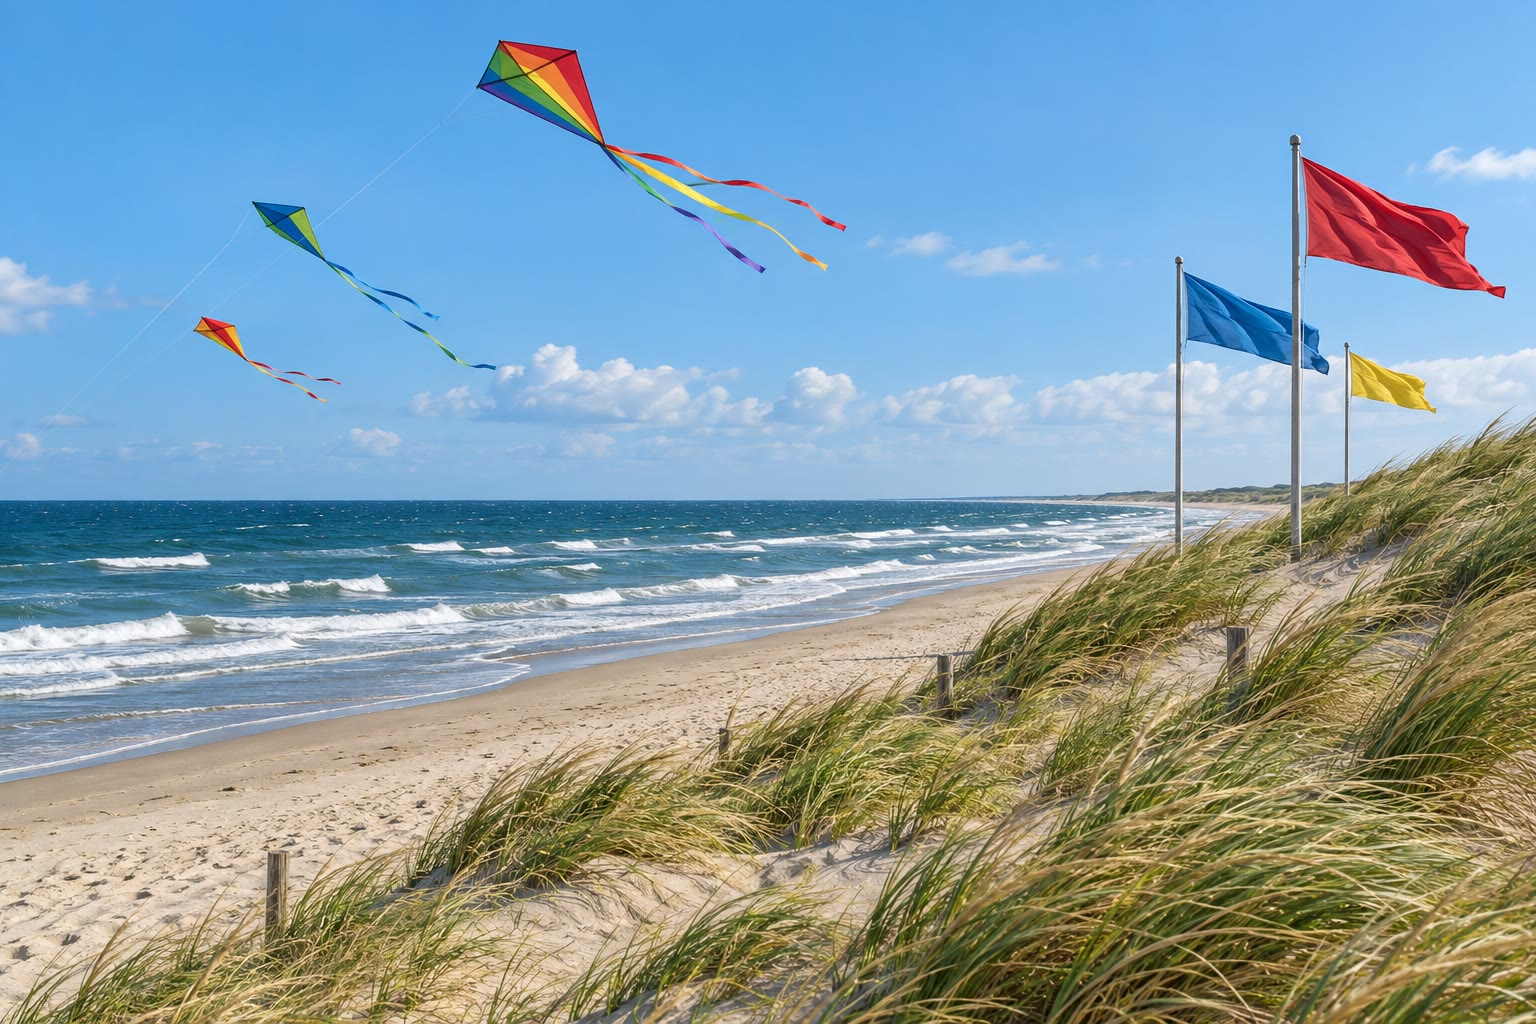
\includegraphics[width=0.55\linewidth]{images/book1/ai/g8-beach-kites.jpg}

{\small Vliegers in de middagwind op een strand (door AI gegenereerde
illustratie van een algemene scène).}
\label{fig:g8:winds-global-circulation:kites}
\end{omfigure}

\section{De algemene winden}

Op de schaal van de hele Aarde gebeurt hetzelfde. Bij de \omterm{def:g3:continents-and-oceans:equator}{evenaar} stijgt de
sterk verwarmde lucht op; ze spreidt zich op hoogte uit naar de \omterm{def:g3:continents-and-oceans:poles}{polen} en
daalt weer rond \ang{30} breedte. Gemiddeld over vele jaren draait de
\omterm{def:g8:the-atmosphere:layers}{troposfeer} van elk \omterm{def:g3:continents-and-oceans:equator}{halfrond} in drie grote \omterm{def:g8:winds-global-circulation:convection-cell}{convectiecellen}: een van de
\omterm{def:g3:continents-and-oceans:equator}{evenaar} tot ongeveer \ang{30}, een van ongeveer \ang{30} tot ongeveer
\ang{60}, en een van ongeveer \ang{60} tot de \omterm{def:g3:continents-and-oceans:poles}{pool}. Meteorologen noemen ze
de hadleycel, de ferrelcel en de poolcel. Hun grenzen verschuiven met de
seizoenen, en de middelste cel is een ruw gemiddelde van vele
voorbijtrekkende \omterm{def:g5:natural-hazards:storm}{stormen}.
% ledger: mo:three-cells, mo:global-circ, nos:doldrums

De winden aan de grond zouden recht van hoge naar lage druk waaien als de
Aarde niet draaide. Omdat de Aarde draait, wordt bewegende lucht
afgebogen: naar rechts op het \omterm{def:g3:continents-and-oceans:equator}{noordelijk halfrond}, naar links op het
\omterm{def:g3:continents-and-oceans:equator}{zuidelijk halfrond}. De lucht die naar de \omterm{def:g3:continents-and-oceans:equator}{evenaar} terugstroomt, komt dus
niet uit het noorden, maar uit het noordoosten op het \omterm{def:g3:continents-and-oceans:equator}{noordelijk halfrond}
en uit het zuidoosten op het \omterm{def:g3:continents-and-oceans:equator}{zuidelijk halfrond}.
% ledger: mo:global-circ, nos:trade-winds

\begin{definition}[De algemene winden]\label{def:g8:winds-global-circulation:global-winds}
De winden aan het oppervlak die in elke breedtegordel het vaakst waaien,
zijn:
\begin{itemize}
  \item de \emph{passaatwinden}\index{passaatwinden}, tussen de \omterm{def:g3:continents-and-oceans:equator}{evenaar} en
        ongeveer \ang{30}, die op het \omterm{def:g3:continents-and-oceans:equator}{noordelijk halfrond} uit het noordoosten
        en op het \omterm{def:g3:continents-and-oceans:equator}{zuidelijk halfrond} uit het zuidoosten waaien;
  \item de \emph{westenwinden}\index{westenwinden}, tussen ongeveer
        \ang{30} en \ang{60}, die uit het westen waaien (uit het zuidwesten
        op het \omterm{def:g3:continents-and-oceans:equator}{noordelijk halfrond}, uit het noordwesten op het zuidelijk);
  \item de \emph{polaire oostenwinden}\index{polaire oostenwinden}, tussen
        ongeveer \ang{60} en de \omterm{def:g3:continents-and-oceans:poles}{polen}, die uit het oosten waaien.
\end{itemize}
\end{definition}
% ledger: nos:trade-winds, mo:three-cells, mo:global-circ

\begin{omfigure}
\begin{tikzpicture}[font=\scriptsize, >={Stealth[length=1.8mm]}]
  \def\R{3}
  \fill[blue!8] (0,0) circle (\R);
  \draw (0,0) circle (\R);
  \draw[black!45] (-\R,0) -- (\R,0);
  \foreach \l in {-60,-30,30,60} {
    \pgfmathsetmacro{\y}{\R*sin(\l)}
    \pgfmathsetmacro{\x}{\R*cos(\l)}
    \draw[black!45, dashed] (-\x,\y) -- (\x,\y);}
  % surface winds: NE trades, SW westerlies, NE polar easterlies (north); mirrored south
  \foreach \x in {-1.8,-0.6,0.6,1.8} {
    \draw[->, omThm, line width=0.9pt] (\x+0.35,0.95) -- (\x-0.35,0.55);
    \draw[->, omThm, line width=0.9pt] (\x+0.35,-0.95) -- (\x-0.35,-0.55);}
  \foreach \x in {-1.2,0,1.2} {
    \draw[->, omDef, line width=0.9pt] (\x-0.35,1.7) -- (\x+0.35,2.02);
    \draw[->, omDef, line width=0.9pt] (\x-0.35,-1.7) -- (\x+0.35,-2.02);}
  \foreach \x in {-0.4,0.4} {
    \draw[->, omMeth, line width=0.9pt] (\x+0.25,2.85) -- (\x-0.25,2.65);
    \draw[->, omMeth, line width=0.9pt] (\x+0.25,-2.85) -- (\x-0.25,-2.65);}
  \node[fill=blue!8, inner sep=1pt] at (0,1.2) {noordoostpassaat};
  \node[fill=blue!8, inner sep=1pt] at (0,-1.2) {zuidoostpassaat};
  \node[fill=blue!8, inner sep=1pt] at (0,2.3) {westenwinden};
  \node[fill=blue!8, inner sep=1pt] at (0,-2.3) {westenwinden};
  \node[anchor=south] at (0,\R+0.05) {polaire oostenwinden};
  \node[anchor=north] at (0,-\R-0.05) {polaire oostenwinden};
  % pressure belts on the left
  \foreach \l/\t in {90/{H: dalende lucht}, 60/{L: stijgende lucht}, 30/{H: dalende lucht, droog, woestijnen}, 0/{L: stijgende lucht, wolken, regen}, -30/{H: dalende lucht, droog, woestijnen}, -60/{L: stijgende lucht}, -90/{H: dalende lucht}} {
    \pgfmathsetmacro{\y}{\R*sin(\l)}
    \pgfmathsetmacro{\x}{\R*cos(\l)}
    \draw[black!40] (-\x-0.05,\y) -- (-3.35,\y);
    \node[anchor=east] at (-3.4,\y) {\t};}
  \foreach \l/\t in {60/{\ang{60} NB}, 30/{\ang{30} NB}, 0/{evenaar}, -30/{\ang{30} ZB}, -60/{\ang{60} ZB}} {
    \pgfmathsetmacro{\y}{\R*sin(\l)}
    \pgfmathsetmacro{\x}{\R*cos(\l)}
    \node[anchor=west, black!60] at (\x+0.05,\y) {\t};}
  % side view of the cells (height to the right), same latitude scale
  \begin{scope}[xshift=5.2cm]
    \draw[->] (0,-\R) -- (0,\R+0.3);
    \draw (0,-\R) -- (1.8,-\R);
    \node[anchor=north, align=center] at (0.9,-\R-0.05) {hoogte in de\\troposfeer $\rightarrow$};
    \foreach \lo/\hi/\cw in {0/30/0, 30/60/1, 60/90/0, -30/0/1, -60/-30/0, -90/-60/1} {
      \pgfmathsetmacro{\ya}{\R*sin(\lo)}
      \pgfmathsetmacro{\yb}{\R*sin(\hi)}
      \pgfmathsetmacro{\yc}{(\ya+\yb)/2}
      \pgfmathsetmacro{\bb}{max(0.09,(\yb-\ya)/2-0.06)}
      \ifnum\cw=0
        \draw[black!70, line width=0.7pt, postaction={decorate}, decoration={markings,
          mark=at position 0.125 with {\arrow{Stealth[length=1.6mm]}}, mark=at position 0.375 with {\arrow{Stealth[length=1.6mm]}},
          mark=at position 0.625 with {\arrow{Stealth[length=1.6mm]}}, mark=at position 0.875 with {\arrow{Stealth[length=1.6mm]}}}]
          (0.9,\yc) ++(0.75,0) arc (0:360:0.75 and \bb);
      \else
        \draw[black!70, line width=0.7pt, postaction={decorate}, decoration={markings,
          mark=at position 0.125 with {\arrow{Stealth[length=1.6mm]}}, mark=at position 0.375 with {\arrow{Stealth[length=1.6mm]}},
          mark=at position 0.625 with {\arrow{Stealth[length=1.6mm]}}, mark=at position 0.875 with {\arrow{Stealth[length=1.6mm]}}}]
          (0.9,\yc) ++(0.75,0) arc (360:0:0.75 and \bb);
      \fi}
  \end{scope}
\end{tikzpicture}

{\small De \omterm{def:g8:winds-global-circulation:circulation}{algemene circulatie}, vereenvoudigd. Links: de gordels van hoge
(H) en lage (L) druk aan de grond. Op de \omterm{def:g3:continents-and-oceans:globe}{globe}: de winden aan het
oppervlak, afgebogen door de draaiing van de Aarde. Rechts: de drie
\omterm{def:g8:winds-global-circulation:convection-cell}{convectiecellen} van elk \omterm{def:g3:continents-and-oceans:equator}{halfrond} van opzij gezien, op dezelfde breedten (de
poolcellen zijn heel dun getekend omdat de poolstrook op de \omterm{def:g3:continents-and-oceans:globe}{globe} smal
is).}
% ledger: mo:three-cells, mo:global-circ, nos:trade-winds, nos:doldrums
\label{fig:g8:winds-global-circulation:cells}
\end{omfigure}

\begin{method}[De algemene wind op een breedte vinden]\label{met:g8:winds-global-circulation:wind}
\begin{enumerate}
  \item Zoek de gordel: van de \omterm{def:g3:continents-and-oceans:equator}{evenaar} tot ongeveer \ang{30}, van \ang{30}
        tot \ang{60}, of van \ang{60} tot de \omterm{def:g3:continents-and-oceans:poles}{pool}.
  \item Zoek in welke richting de lucht in die gordel aan de grond stroomt:
        naar de \omterm{def:g3:continents-and-oceans:equator}{evenaar} in de eerste en de laatste gordel, naar de \omterm{def:g3:continents-and-oceans:poles}{pool} in
        de middelste.
  \item Buig deze stroming af: naar rechts op het \omterm{def:g3:continents-and-oceans:equator}{noordelijk halfrond}, naar
        links op het \omterm{def:g3:continents-and-oceans:equator}{zuidelijk halfrond}.
  \item Zeg waar de wind vandaan komt: winden worden genoemd naar de
        richting \emph{waaruit} ze waaien.
\end{enumerate}
\end{method}

\begin{example}[De wind op \ang{40} zuiderbreedte]\label{ex:g8:winds-global-circulation:40s}
Op \ang{40} ZB zijn we in de middelste gordel, tussen \ang{30} en
\ang{60}. Daar stroomt de lucht aan de grond naar de \omterm{def:g3:continents-and-oceans:poles}{pool}, dat wil zeggen
naar het zuiden. Op het \omterm{def:g3:continents-and-oceans:equator}{zuidelijk halfrond} wordt ze naar links afgebogen:
voor lucht die naar het zuiden gaat, is links het oosten, dus beweegt de
lucht uiteindelijk naar het zuidoosten. Ze komt dus uit het noordwesten:
het is een van de \omterm{def:g8:winds-global-circulation:global-winds}{westenwinden}, uit het noordwesten.
\end{example}
% ledger: mo:three-cells, mo:global-circ

Bij de \omterm{def:g3:continents-and-oceans:equator}{evenaar}, waar de \omterm{def:g8:winds-global-circulation:global-winds}{passaatwinden} van de twee \omterm{def:g3:continents-and-oceans:equator}{halfronden} elkaar
ontmoeten, gaan de winden liggen: zeelieden noemden deze windstille gordel
de \emph{stiltegordel}. De warme, vochtige lucht stijgt daar op, koelt af
en geeft aanhoudende buien en onweer. Rond \ang{30}, onder de dalende
lucht, zijn de winden zwak en is \omterm{def:g4:clouds-rain-snow:precipitation}{regen} zeldzaam.
% ledger: nos:doldrums

\begin{definition}[Algemene circulatie van de atmosfeer]\label{def:g8:winds-global-circulation:circulation}
De \emph{algemene circulatie}\index{algemene circulatie} van de atmosfeer
is de grootschalige beweging van lucht rond de planeet, die zichtbaar wordt
als je de winden over vele jaren middelt. Ze voert warmte van de \omterm{def:g3:continents-and-oceans:equator}{evenaar}
naar de \omterm{def:g3:continents-and-oceans:poles}{polen}, en waterdamp van de ene breedtegordel naar de andere.
\end{definition}
% ledger: mo:global-circ

\section{De algemene circulatie en de klimaatzones}

De \omterm{def:g8:winds-global-circulation:circulation}{algemene circulatie} verklaart veel van de \omterm{def:g2:drawing-to-map:map}{kaart} van de klimaten. Waar
lucht opstijgt, bij de \omterm{def:g3:continents-and-oceans:equator}{evenaar}, koelt ze af en wordt haar waterdamp
\omterm{def:g4:clouds-rain-snow:cloud}{wolken}: \omterm{def:g4:clouds-rain-snow:precipitation}{regen} valt vaak, en er groeien \omterm{def:g5:weather-and-climate:rainforest}{regenwouden}. Waar de lucht daalt,
rond \ang{30} noorder- en \omterm{def:g6:latitude-longitude:latitude}{zuiderbreedte}, warmt ze op terwijl ze daalt,
drogen haar \omterm{def:g4:clouds-rain-snow:cloud}{wolken} op en is \omterm{def:g4:clouds-rain-snow:precipitation}{regen} zeldzaam: de grote hete \omterm{def:g5:weather-and-climate:desert}{woestijnen}, zoals
de Sahara, liggen in deze gordels. Op de gematigde breedten brengen de
\omterm{def:g8:winds-global-circulation:global-winds}{westenwinden} de ene \omterm{def:g5:natural-hazards:storm}{storm} na de andere, met \omterm{def:g4:clouds-rain-snow:precipitation}{regen} in alle seizoenen.
% ledger: nos:doldrums, mo:three-cells, mo:global-circ

\begin{omfigure}
\begin{minipage}[c]{0.42\linewidth}\centering
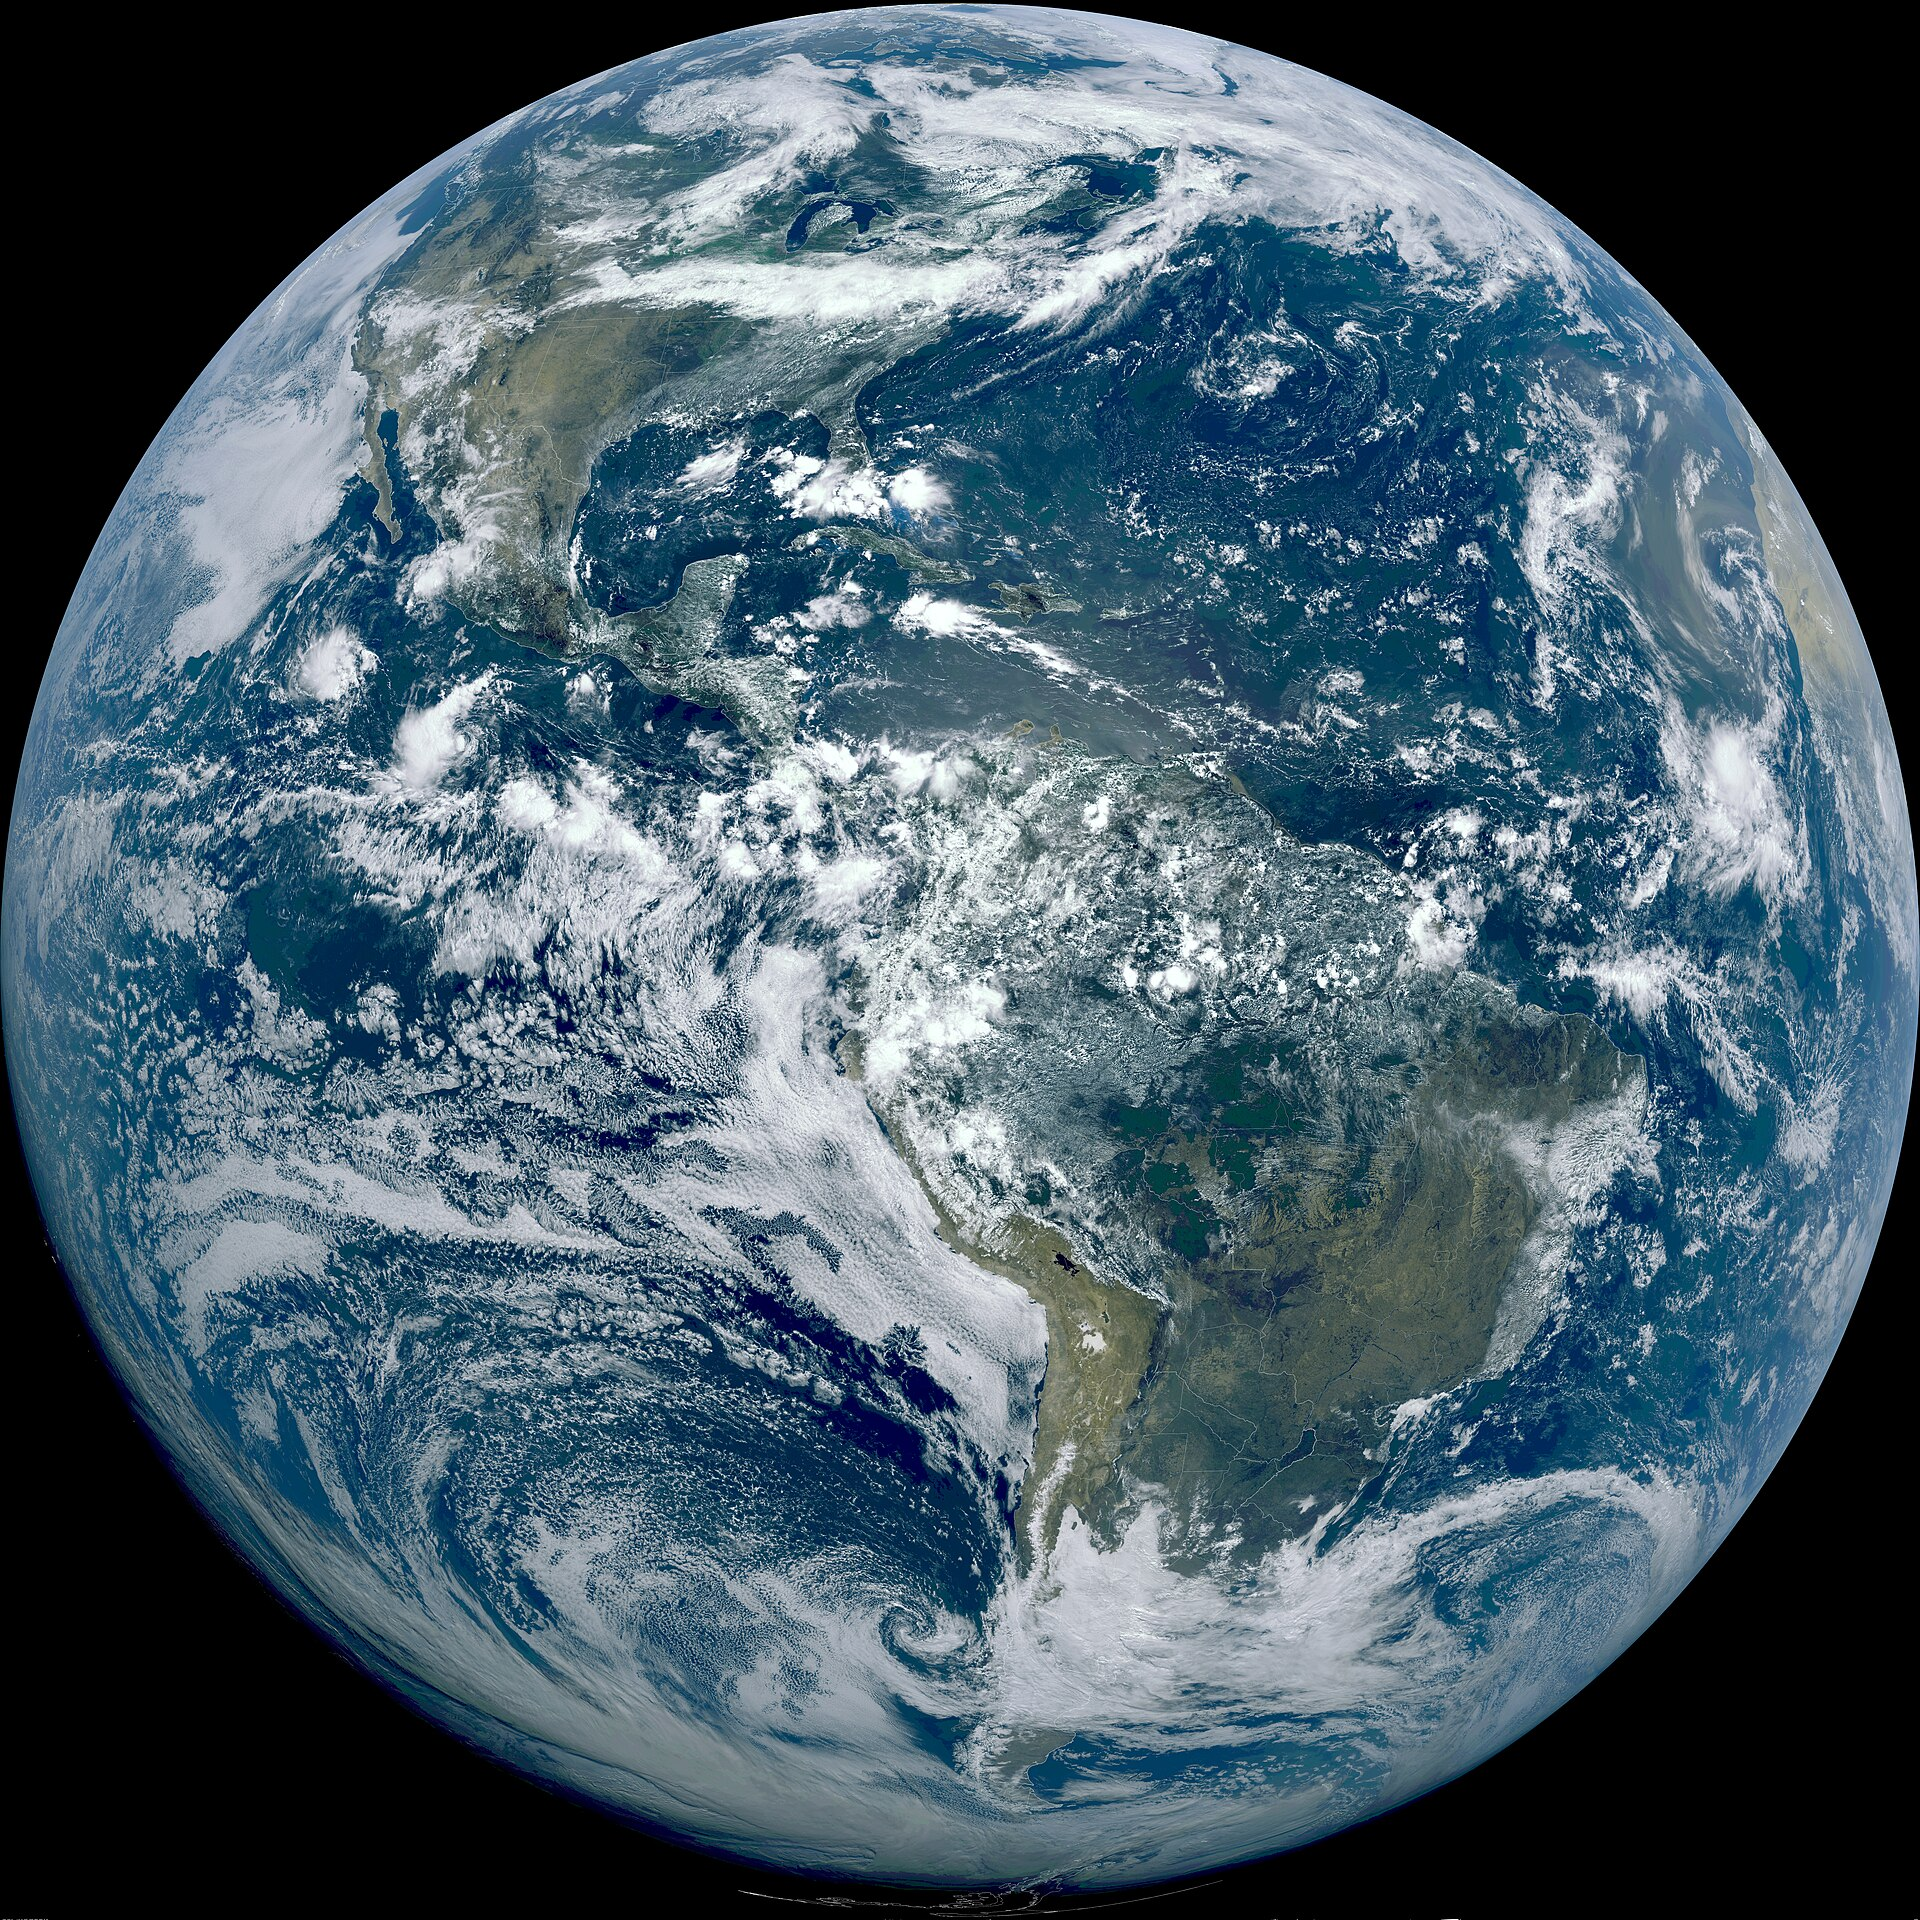
\includegraphics[width=\linewidth]{images/book1/g8-goes-full-disk.jpg}
\end{minipage}\hfill
\begin{minipage}[c]{0.54\linewidth}\raggedright
{\small Noord- en Zuid-Amerika gezien door de weersatelliet GOES-16, hoog
boven de \omterm{def:g3:continents-and-oceans:equator}{evenaar}, op 26~juli 2022. Boven de tropen en het Amazoneregenwoud,
waar warme, vochtige lucht opstijgt, zijn veel \omterm{def:g4:clouds-rain-snow:cloud}{wolken} ontstaan; ver naar
het zuiden, in de zuidelijke winter, wervelen de \omterm{def:g5:natural-hazards:storm}{stormen} van de
\omterm{def:g8:winds-global-circulation:global-winds}{westenwinden} boven de \omterm{def:g2:water-on-earth:ocean}{oceaan}. NOAA (publiek domein, via Wikimedia
Commons).}
\end{minipage}
% ledger: commons:goes16, nos:doldrums
\label{fig:g8:winds-global-circulation:goes}
\end{omfigure}

\begin{example}[Vier steden, vier gordels]\label{ex:g8:winds-global-circulation:four-towns}
De vier steden van de \omterm{def:g5:weather-and-climate:climate-chart}{klimaatdiagrammen} van \cref{ch:g5:weather-and-climate}
liggen allemaal op het \omterm{def:g3:continents-and-oceans:equator}{noordelijk halfrond}, op heel verschillende breedten.
Hun jaarlijkse \omterm{def:g4:clouds-rain-snow:precipitation}{regen} en \omterm{def:g4:clouds-rain-snow:precipitation}{sneeuw} volgen de gordels van de \omterm{def:g8:winds-global-circulation:circulation}{algemene circulatie}
(diagram hieronder). Hilo, op \ang{20}\,NB, ligt op een eiland in de
passaatgordel, midden in de \omterm{def:g2:water-on-earth:ocean}{oceaan}, waar de \omterm{def:g8:winds-global-circulation:global-winds}{passaatwinden} waterdamp
opnemen: er valt daar ongeveer \qty{3000}{mm} per jaar. Phoenix, op
\ang{33}\,NB, ligt dicht bij \ang{30}, onder de dalende lucht: minder dan
\qty{200}{mm}. Seattle, op \ang{47}\,NB, ligt in de \omterm{def:g8:winds-global-circulation:global-winds}{westenwinden}, waarvan
de \omterm{def:g5:natural-hazards:storm}{stormen} ongeveer \qty{1000}{mm} per jaar brengen, het meeste van de
herfst tot de lente. Utqiaġvik, op \ang{71}\,NB, ligt onder de koude lucht
die bij de \omterm{def:g3:continents-and-oceans:poles}{pool} daalt: minder dan \qty{150}{mm}, een koude \omterm{def:g5:weather-and-climate:desert}{woestijn}.
% ledger: data:b1-noaa-normals (totals from figdata/grade-5/climate_charts.py, re-read in figdata/grade-8/rain_by_belt.py), mo:three-cells, nos:doldrums
\end{example}

\begin{omfigure}
\begin{tikzpicture}
\begin{axis}[xbar, width=0.82\linewidth, height=6.4cm, bar width=9pt,
  xmin=0, xmax=3600, ymin=0, ymax=90, ytick={0,30,60,90},
  yticklabels={$0^\circ$, $30^\circ$\,NB, $60^\circ$\,NB, $90^\circ$\,NB},
  xlabel={regen en sneeuw in een jaar (mm)}, ylabel={breedte},
  axis x line=bottom, axis y line=left, axis line style={-},
  tick label style={font=\scriptsize}, label style={font=\small},
  xtick={0,1000,2000,3000}, scaled x ticks=false, clip=false,
  point meta=explicit symbolic, nodes near coords,
  nodes near coords style={font=\scriptsize, anchor=west}]
  \draw[black!35, dashed] (axis cs:0,30) -- (axis cs:3600,30);
  \draw[black!35, dashed] (axis cs:0,60) -- (axis cs:3600,60);
  \node[font=\scriptsize, black!60, anchor=south east] at (axis cs:3600,1) {stijgende lucht: regen};
  \node[font=\scriptsize, black!60, anchor=south east] at (axis cs:3600,30) {dalende lucht: droog};
  \node[font=\scriptsize, black!60, anchor=south east] at (axis cs:3600,60) {stijgende lucht: regen};
  \node[font=\scriptsize, black!60, anchor=north east] at (axis cs:3600,90) {dalende lucht: droog};
  \addplot[fill=blue!35, draw=blue!60!black] table[x=total_mm, y=lat, meta=name] {figdata/out/grade-8-rain_by_belt-stations.dat};
\end{axis}
\end{tikzpicture}

{\small Jaarlijkse \omterm{def:g4:clouds-rain-snow:precipitation}{regen} en \omterm{def:g4:clouds-rain-snow:precipitation}{sneeuw} (gemiddelden 1991--2020) van de vier
steden van de \omterm{def:g5:weather-and-climate:climate-chart}{klimaatdiagrammen}, geplaatst op hun breedte. De natte steden
liggen waar lucht opstijgt, bij de \omterm{def:g3:continents-and-oceans:equator}{evenaar} en rond \ang{60}; de droge waar
ze daalt, rond \ang{30} en bij de \omterm{def:g3:continents-and-oceans:poles}{pool}. Klimaatnormalen van de NOAA.}
% ledger: data:b1-noaa-normals, mo:three-cells (figdata/grade-8/rain_by_belt.py)
\end{omfigure}

Vier steden zijn maar vier punten: \omterm{def:g1:landscapes-around-us:landform}{bergen}, \omterm{def:g1:landscapes-around-us:water}{kusten} en koude of warme \omterm{def:g2:water-on-earth:ocean}{zeeën}
veranderen ook hoeveel \omterm{def:g4:clouds-rain-snow:precipitation}{regen} een plek krijgt. De gordels geven het grote
patroon van de \omterm{def:g2:drawing-to-map:map}{kaart} van de klimaten, niet de \omterm{def:g4:clouds-rain-snow:precipitation}{regen} van elke stad.

\section{Oefeningen}

\begin{exercise}[$\star$]\label{exo:g8:winds-global-circulation:1}
Noem de algemene wind die het vaakst waait: (a) op \ang{15} NB; (b) op
\ang{45} ZB; (c) op \ang{75} NB; (d) op \ang{20} ZB. Geef telkens zijn
richting.
\end{exercise}

\begin{exercise}[$\star$]\label{exo:g8:winds-global-circulation:2}
Maak elke zin af. (a) Warme lucht \dots\ en koude lucht \dots. (b) Onder
stijgende lucht is de druk aan de grond \dots. (c) Aan de grond waait de
wind van \dots\ druk naar \dots\ druk. (d) Op het \omterm{def:g3:continents-and-oceans:equator}{noordelijk halfrond} buigt
de draaiing van de Aarde bewegende lucht af naar \dots.
\end{exercise}

\begin{exercise}[$\star$]\label{exo:g8:winds-global-circulation:3}
Waar of niet waar? Verbeter de onware zinnen. (a) Een \omterm{def:g8:winds-global-circulation:breezes}{zeewind} waait van
het land naar de \omterm{def:g2:water-on-earth:ocean}{zee}. (b) Overdag warmt het land sneller op dan de \omterm{def:g2:water-on-earth:ocean}{zee}.
(c) De \omterm{def:g8:winds-global-circulation:global-winds}{passaatwinden} waaien uit het westen. (d) Veel grote \omterm{def:g5:weather-and-climate:desert}{woestijnen}
liggen rond \ang{30} breedte.
\end{exercise}

\begin{exercise}[$\star$]\label{exo:g8:winds-global-circulation:4}
Teken een \omterm{def:g1:landscapes-around-us:water}{kust} met de \omterm{def:g2:water-on-earth:ocean}{zee} links en het land rechts. Voeg de Zon toe en
teken dan met pijlen de kringloop van de lucht van de \omterm{def:g8:winds-global-circulation:breezes}{zeewind}. Zet H en L
waar de druk aan de grond hoog en laag is.
\end{exercise}

\begin{exercise}[$\star\star$]\label{exo:g8:winds-global-circulation:5}
Gebruik de tabel met bundels in dit hoofdstuk. (a) Hoeveel meer grond
bedekt een bundel op \ang{45} dan bij de \omterm{def:g3:continents-and-oceans:equator}{evenaar}? (b) Welk percentage van
de energie bij de \omterm{def:g3:continents-and-oceans:equator}{evenaar} krijgt elke vierkante meter op \ang{60}? (c) Op
\ang{75}? (d) Leg in één zin uit waarom het bij de \omterm{def:g3:continents-and-oceans:poles}{polen} koud is.
\end{exercise}

\begin{exercise}[$\star\star$]\label{exo:g8:winds-global-circulation:6}
Een boot vaart pal naar het zuiden door het noordelijk en daarna het
\omterm{def:g3:continents-and-oceans:equator}{zuidelijk halfrond}. (a) Welke winden komt hij tegen, in volgorde, van
\ang{70} NB tot \ang{70} ZB? (b) Waar zal hij waarschijnlijk windstilte en
veel buien vinden? (c) Waar zijn de winden zwak en is \omterm{def:g4:clouds-rain-snow:precipitation}{regen} zeldzaam?
\end{exercise}

\begin{exercise}[$\star\star$]\label{exo:g8:winds-global-circulation:7}
Op een strand is het om 15~uur \qty{31}{\degreeCelsius} op het \omterm{def:g3:stones-pebbles-sand:sand}{zand} en
\qty{22}{\degreeCelsius} boven de \omterm{def:g2:water-on-earth:ocean}{zee}. Om 3~uur 's nachts is het
\qty{17}{\degreeCelsius} op het land en \qty{21}{\degreeCelsius} boven de
\omterm{def:g2:water-on-earth:ocean}{zee}. (a) Wat is om 15~uur warmer? Welke kant op waait de wind? (b) En om
3~uur 's nachts? (c) Hoeveel graden verandert de temperatuur van het land
tussen de twee tijdstippen? En die van de \omterm{def:g2:water-on-earth:ocean}{zee}? (d) Verklaar het verschil.
\end{exercise}

\begin{exercise}[$\star\star$]\label{exo:g8:winds-global-circulation:8}
Lucht stroomt van de hogedrukgordel rond \ang{30} NB naar de \omterm{def:g3:continents-and-oceans:equator}{evenaar}.
(a) Uit welke richting zou ze waaien zonder de draaiing van de Aarde?
(b) Naar welke kant buigt de draaiing haar af op dit \omterm{def:g3:continents-and-oceans:equator}{halfrond}? (c) Uit
welke richting waait ze dan? (d) Beantwoord dezelfde drie vragen voor de
lucht die vanaf \ang{30} ZB naar de \omterm{def:g3:continents-and-oceans:equator}{evenaar} stroomt.
\end{exercise}

\begin{exercise}[$\star\star$]\label{exo:g8:winds-global-circulation:9}
Leg stap voor stap uit waarom het bij de \omterm{def:g3:continents-and-oceans:equator}{evenaar} zo vaak regent: gebruik de
woorden \emph{verwarmd}, \emph{stijgt}, \emph{koelt af}, \emph{\omterm{def:g4:clouds-rain-snow:cloud}{wolken}}. Leg
daarna uit waarom er rond \ang{25} NB in Noord-Afrika een \omterm{def:g5:weather-and-climate:desert}{woestijn} ligt:
gebruik de woorden \emph{daalt}, \emph{hoge druk}, \emph{droog}.
\end{exercise}

\begin{exercise}[$\star\star$]\label{exo:g8:winds-global-circulation:10}
Een zeilschip vertrekt uit een haven op \ang{40} NB aan de westkust van
Europa naar het Caribisch gebied, op \ang{15} NB. (a) Welke wind zou het op
\ang{40} NB tegenkomen? Zou die het schip helpen naar het westen te varen?
(b) Waarom zou het schip eerst naar het zuiden moeten varen? (c) Welke wind
voert het naar het westen, en tussen welke breedten? (d) Naar welke wind
moet het schip voor de terugreis naar Europa zoeken, en op welke breedte?
\end{exercise}

\begin{exercise}[$\star\star\star$]\label{exo:g8:winds-global-circulation:11}
Op breedte $L$ bedekt een bundel zonlicht om 12 uur 's middags op een
equinox $1 \div
\cos L$ keer zoveel grond als bij de \omterm{def:g3:continents-and-oceans:equator}{evenaar} (op een rekenmachine:
$\cos 60^\circ = 0.5$). (a) Controleer de waarde voor \ang{60}. (b) Controleer
met $\cos 30^\circ \approx 0.866$ de waarde voor \ang{30}, afgerond op twee
decimalen. (c) Stel dat een plat liggend zonnepaneel op die dag om 12 uur
's middags bij de \omterm{def:g3:continents-and-oceans:equator}{evenaar} \qty{1000}{W} per vierkante meter krijgt. Hoeveel
zou hetzelfde paneel ongeveer krijgen op \ang{30}? Op \ang{60}?
\end{exercise}

\begin{exercise}[$\star\star\star$]\label{exo:g8:winds-global-circulation:12}
Op elk \omterm{def:g3:continents-and-oceans:equator}{halfrond} heeft de \omterm{def:g8:winds-global-circulation:circulation}{algemene circulatie} drie cellen. (a) Teken een
zijaanzicht van het \omterm{def:g3:continents-and-oceans:equator}{noordelijk halfrond}, met de \omterm{def:g3:continents-and-oceans:equator}{evenaar} onderaan en de \omterm{def:g3:continents-and-oceans:poles}{pool}
bovenaan, en de drie cellen als kringlopen; geef aan waar de lucht opstijgt
en waar ze daalt. (b) Geef de gordels van hoge en lage druk aan de grond
aan. (c) Voeg de winden aan het oppervlak van elke cel toe, naar rechts
afgebogen. (d) Leg met je tekening uit waarom de \omterm{def:g8:winds-global-circulation:global-winds}{westenwinden} naar het
noordoosten waaien.
\end{exercise}

\section{Probleem: Zeilen met de passaatwinden}

\begin{problem}[{Weekendprobleem --- een zeilschip steekt met de
noordoostpassaat de Atlantische Oceaan over van Kaapverdië naar Barbados; de
route wordt op de kaart gemeten, de wind wordt afgelezen, en de duur van de
overtocht wordt berekend}]
\label{pb:g8:winds-global-circulation:1}
% ledger: data:b1-ne-places, earth:Rmean, nos:trade-winds (figdata/grade-8/trade_route.py; the speed is exercise data)
Een zeilschip vertrekt uit Praia, op de Kaapverdische Eilanden, naar
Bridgetown, op Barbados. De \omterm{def:g2:drawing-to-map:map}{kaart} toont de route en de passaatwind.

\begin{center}
\begin{tikzpicture}
\begin{axis}[ommap, width=12cm, xmin=-75, xmax=-5, ymin=0, ymax=35, axis equal image,
  xtick={-70,-60,-50,-40,-30,-20,-10}, ytick={0,10,20,30},
  tick label style={font=\scriptsize},
  xlabel={lengte (negatief = west)}, ylabel={breedte (noord)},
  label style={font=\small}, clip mode=individual]
  \addplot[fill=omLithAlluv, draw=black!60, line width=0.3pt] table {figdata/out/grade-8-trade_route-land.dat};
  \addplot[quiver={u=\thisrow{dlon}, v=\thisrow{dlat}}, -{Stealth[length=1.6mm]}, omThm!80, line width=0.7pt]
    table[x=lon, y=lat] {figdata/out/grade-8-trade_route-trades.dat};
  \addplot[omDef, line width=1.3pt, dashed] table {figdata/out/grade-8-trade_route-route.dat};
  \addplot[only marks, mark=*, mark size=2pt, black] table[x=lon, y=lat] {figdata/out/grade-8-trade_route-ports.dat};
  \node[anchor=north, font=\scriptsize\bfseries, fill=white, inner sep=1pt] at (axis cs:-59.6,12.2) {Bridgetown};
  \node[anchor=south, font=\scriptsize\bfseries, fill=white, inner sep=1pt] at (axis cs:-23.5,15.8) {Praia};
\end{axis}
\end{tikzpicture}
\end{center}

\noindent\textbf{Deel I --- De route.}\par\nopagebreak
\begin{enumerate}[beginpenalty=10000]
  \item Praia ligt op \ang{14.9} NB, \ang{23.5} WL; Bridgetown op
        \ang{13.1} NB, \ang{59.6} WL. Hoeveel lengtegraden liggen ertussen?
  \item Beide havens liggen dicht bij \ang{14} NB. Langs deze \omterm{def:g6:latitude-longitude:latitude}{breedtecirkel}
        meet één \omterm{def:g6:latitude-longitude:longitude}{lengtegraad} ongeveer \qty{108}{km}. Ongeveer hoeveel
        kilometer is de overtocht? Rond af op honderdtallen.
  \item Precies gemeten op de ronde Aarde is de kortste route
        \qty{3896}{km}. Is het antwoord op vraag 2 een goede schatting?
  \item Liggen de havens in de gordel van de \omterm{def:g8:winds-global-circulation:global-winds}{passaatwinden}? Leg uit.
\end{enumerate}

\noindent\textbf{Deel II --- De wind.}\par\nopagebreak
\begin{enumerate}[resume, beginpenalty=10000]
  \item Uit welke richting waait de passaatwind hier?
  \item Het schip vaart naar het westen. Duwt de wind het vooruit,
        achteruit of opzij? Leg uit met de \omterm{def:g2:drawing-to-map:map}{kaart}.
  \item Waarom waait de passaatwind bijna elke dag van de overtocht in
        dezelfde richting?
  \item Waarom moet de kapitein op de terugweg naar Europa niet proberen
        langs \ang{14} NB naar het oosten te varen?
\end{enumerate}

\noindent\textbf{Deel III --- De overtocht.}\par\nopagebreak
\begin{enumerate}[resume, beginpenalty=10000]
  \item Stel dat het schip gemiddeld \qty{7}{km} per uur aflegt. Hoeveel
        kilometer legt het af in een dag van 24 uur?
  \item Als de wind onderweg 3 dagen ging liggen, hoeveel kilometer
        voortgang zou het schip dan verliezen?
  \item Hoeveel dagen heeft het schip met een gestage passaatwind nodig voor
        \qty{3896}{km}? Rond af op één decimaal.
  \item Hoe lang duurt de overtocht, afgerond op een hele dag? Is dat meer
        of minder dan een maand?
\end{enumerate}
\end{problem}
